\documentclass[twoside]{book}

% Packages required by doxygen
\usepackage{fixltx2e}
\usepackage{calc}
\usepackage{doxygen}
\usepackage[export]{adjustbox} % also loads graphicx
\usepackage{graphicx}
\usepackage[utf8]{inputenc}
\usepackage{makeidx}
\usepackage{multicol}
\usepackage{multirow}
\PassOptionsToPackage{warn}{textcomp}
\usepackage{textcomp}
\usepackage[nointegrals]{wasysym}
\usepackage[table]{xcolor}

% Font selection
\usepackage[T1]{fontenc}
\usepackage[scaled=.90]{helvet}
\usepackage{courier}
\usepackage{amssymb}
\usepackage{sectsty}
\renewcommand{\familydefault}{\sfdefault}
\allsectionsfont{%
  \fontseries{bc}\selectfont%
  \color{darkgray}%
}
\renewcommand{\DoxyLabelFont}{%
  \fontseries{bc}\selectfont%
  \color{darkgray}%
}
\newcommand{\+}{\discretionary{\mbox{\scriptsize$\hookleftarrow$}}{}{}}

% Page & text layout
\usepackage{geometry}
\geometry{%
  a4paper,%
  top=2.5cm,%
  bottom=2.5cm,%
  left=2.5cm,%
  right=2.5cm%
}
\tolerance=750
\hfuzz=15pt
\hbadness=750
\setlength{\emergencystretch}{15pt}
\setlength{\parindent}{0cm}
\setlength{\parskip}{3ex plus 2ex minus 2ex}
\makeatletter
\renewcommand{\paragraph}{%
  \@startsection{paragraph}{4}{0ex}{-1.0ex}{1.0ex}{%
    \normalfont\normalsize\bfseries\SS@parafont%
  }%
}
\renewcommand{\subparagraph}{%
  \@startsection{subparagraph}{5}{0ex}{-1.0ex}{1.0ex}{%
    \normalfont\normalsize\bfseries\SS@subparafont%
  }%
}
\makeatother

% Headers & footers
\usepackage{fancyhdr}
\pagestyle{fancyplain}
\fancyhead[LE]{\fancyplain{}{\bfseries\thepage}}
\fancyhead[CE]{\fancyplain{}{}}
\fancyhead[RE]{\fancyplain{}{\bfseries\leftmark}}
\fancyhead[LO]{\fancyplain{}{\bfseries\rightmark}}
\fancyhead[CO]{\fancyplain{}{}}
\fancyhead[RO]{\fancyplain{}{\bfseries\thepage}}
\fancyfoot[LE]{\fancyplain{}{}}
\fancyfoot[CE]{\fancyplain{}{}}
\fancyfoot[RE]{\fancyplain{}{\bfseries\scriptsize Generated by Doxygen }}
\fancyfoot[LO]{\fancyplain{}{\bfseries\scriptsize Generated by Doxygen }}
\fancyfoot[CO]{\fancyplain{}{}}
\fancyfoot[RO]{\fancyplain{}{}}
\renewcommand{\footrulewidth}{0.4pt}
\renewcommand{\chaptermark}[1]{%
  \markboth{#1}{}%
}
\renewcommand{\sectionmark}[1]{%
  \markright{\thesection\ #1}%
}

% Indices & bibliography
\usepackage{natbib}
\usepackage[titles]{tocloft}
\setcounter{tocdepth}{3}
\setcounter{secnumdepth}{5}
\makeindex

% Hyperlinks (required, but should be loaded last)
\usepackage{ifpdf}
\ifpdf
  \usepackage[pdftex,pagebackref=true]{hyperref}
\else
  \usepackage[ps2pdf,pagebackref=true]{hyperref}
\fi
\hypersetup{%
  colorlinks=true,%
  linkcolor=blue,%
  citecolor=blue,%
  unicode%
}

% Custom commands
\newcommand{\clearemptydoublepage}{%
  \newpage{\pagestyle{empty}\cleardoublepage}%
}

\usepackage{caption}
\captionsetup{labelsep=space,justification=centering,font={bf},singlelinecheck=off,skip=4pt,position=top}

%===== C O N T E N T S =====

\begin{document}

% Titlepage & ToC
\hypersetup{pageanchor=false,
             bookmarksnumbered=true,
             pdfencoding=unicode
            }
\pagenumbering{roman}
\begin{titlepage}
\vspace*{7cm}
\begin{center}%
{\Large Actividad 2 }\\
\vspace*{1cm}
{\large Generated by Doxygen 1.8.11}\\
\end{center}
\end{titlepage}
\clearemptydoublepage
\tableofcontents
\clearemptydoublepage
\pagenumbering{arabic}
\hypersetup{pageanchor=true}

%--- Begin generated contents ---
\chapter{Práctica 5}
\label{md_README}
\hypertarget{md_README}{}
\begin{quote}
Martín Molina Álvarez \end{quote}


\begin{quote}
Víctor Malvárez Filgueira \end{quote}


\subsection*{Modo de empleo}


\begin{DoxyEnumerate}
\item Compilar los {\ttfamily .java}.
\item Ir al directorio donde están los {\ttfamily .class}.
\item Abrir el \hyperlink{classServidor}{Servidor} con los argumentos necesarios\+:
\begin{DoxyItemize}
\item puerto
\item divisiones
\item x\+Centro
\item y\+Centro
\item tamaño
\item iteraciones
\item archivo
\end{DoxyItemize}
\item Ejemplo\+: {\ttfamily java \hyperlink{classServidor}{Servidor} 3000 16 512 512 1024 512 imagen.\+pgm}
\item Abrir los clientes\+: {\ttfamily java \hyperlink{classCliente}{Cliente} ...} Los argumentos son\+:
\begin{DoxyItemize}
\item hostname\+: la dirección del servidor
\item puerto
\item n\+Clientes\+: Opcional.
\end{DoxyItemize}
\item Ejemplo\+: {\ttfamily java \hyperlink{classCliente}{Cliente} localhost 3000 16}
\end{DoxyEnumerate}

\subsection*{Arquitectura}

\subsubsection*{\hyperlink{classServidor}{Servidor}}

Clase principal del servidor que se encarga de abrir las conexiones con los clientes y de gestionar el proceso de organización y control de las colas.

\subsubsection*{\hyperlink{classServidorThread}{Servidor\+Thread}}

Clase cuyas instancias son creadas cada vez que se conecta un nueco cliente. Gestiona y controla una conexión individual con un cliente.

\subsubsection*{\hyperlink{classCliente}{Cliente}}

Clase cuyas instancias son creadas una vez que se ha abierto el servidor. Hacen las llamadas al algoritmo de \hyperlink{classMandelbrot}{Mandelbrot}.

\subsubsection*{\hyperlink{classTrabajo}{Trabajo}}

Clase que contiene los atributos necesarios para procesar una región de la imagen del \hyperlink{classMandelbrot}{Mandelbrot}.

\subsubsection*{Acción}

Clase vehicular para comunicarse entre \hyperlink{classCliente}{Cliente} y \hyperlink{classServidor}{Servidor}.

\subsubsection*{\hyperlink{classMandelbrot}{Mandelbrot}}

Clase cuyo método implementa el algoritmo de \hyperlink{classMandelbrot}{Mandelbrot}.

\subsubsection*{\hyperlink{classPGM}{P\+GM}}

Clase que se encarga de la creación de imágenes con el mismo formato que el nombre de la clase y escribe matrices de colores en formato R\+GB. 
\chapter{Hierarchical Index}
\section{Class Hierarchy}
This inheritance list is sorted roughly, but not completely, alphabetically\+:\begin{DoxyCompactList}
\item \contentsline{section}{Mandelbrot}{\pageref{classMandelbrot}}{}
\item \contentsline{section}{P\+GM}{\pageref{classPGM}}{}
\item Runnable\begin{DoxyCompactList}
\item \contentsline{section}{Cliente}{\pageref{classCliente}}{}
\item \contentsline{section}{Servidor}{\pageref{classServidor}}{}
\item \contentsline{section}{Servidor\+Thread}{\pageref{classServidorThread}}{}
\end{DoxyCompactList}
\item Serializable\begin{DoxyCompactList}
\item \contentsline{section}{Accion}{\pageref{classAccion}}{}
\item \contentsline{section}{Trabajo}{\pageref{classTrabajo}}{}
\end{DoxyCompactList}
\end{DoxyCompactList}

\chapter{Class Index}
\section{Class List}
Here are the classes, structs, unions and interfaces with brief descriptions\+:\begin{DoxyCompactList}
\item\contentsline{section}{\hyperlink{classAccion}{Accion} \\*Clase que se utiliza para enviar los objetos entre servidor-\/cliente }{\pageref{classAccion}}{}
\item\contentsline{section}{\hyperlink{classCliente}{Cliente} \\*Implementa la conexión individual con el \hyperlink{classServidor}{Servidor} y realiza las acciones oportunas con los objetos \hyperlink{classTrabajo}{Trabajo} }{\pageref{classCliente}}{}
\item\contentsline{section}{\hyperlink{classMandelbrot}{Mandelbrot} \\*Implementa el método necesario para crear un conjunto de \hyperlink{classMandelbrot}{Mandelbrot} }{\pageref{classMandelbrot}}{}
\item\contentsline{section}{\hyperlink{classPGM}{P\+GM} \\*Implementa el tratamiento de archivos \hyperlink{classPGM}{P\+GM} a partir de matrices de Color }{\pageref{classPGM}}{}
\item\contentsline{section}{\hyperlink{classServidor}{Servidor} \\*Implementa la clase \hyperlink{classServidor}{Servidor} que gestiona todas las conexiones y los trabajos }{\pageref{classServidor}}{}
\item\contentsline{section}{\hyperlink{classServidorThread}{Servidor\+Thread} \\*Clase que se encarga de gestionar individualmente cada conexión con el cliente en el servidor }{\pageref{classServidorThread}}{}
\item\contentsline{section}{\hyperlink{classTrabajo}{Trabajo} \\*Contiene los argumentos necesarios para procesar el conjunto de \hyperlink{classMandelbrot}{Mandelbrot} y ofrece una estructura para guardar los resultados }{\pageref{classTrabajo}}{}
\end{DoxyCompactList}

\chapter{File Index}
\section{File List}
Here is a list of all files with brief descriptions\+:\begin{DoxyCompactList}
\item\contentsline{section}{src/\hyperlink{Accion_8java}{Accion.\+java} }{\pageref{Accion_8java}}{}
\item\contentsline{section}{src/\hyperlink{Cliente_8java}{Cliente.\+java} }{\pageref{Cliente_8java}}{}
\item\contentsline{section}{src/\hyperlink{Mandelbrot_8java}{Mandelbrot.\+java} }{\pageref{Mandelbrot_8java}}{}
\item\contentsline{section}{src/\hyperlink{PGM_8java}{P\+G\+M.\+java} }{\pageref{PGM_8java}}{}
\item\contentsline{section}{src/\hyperlink{Servidor_8java}{Servidor.\+java} }{\pageref{Servidor_8java}}{}
\item\contentsline{section}{src/\hyperlink{ServidorThread_8java}{Servidor\+Thread.\+java} }{\pageref{ServidorThread_8java}}{}
\item\contentsline{section}{src/\hyperlink{Trabajo_8java}{Trabajo.\+java} }{\pageref{Trabajo_8java}}{}
\end{DoxyCompactList}

\chapter{Class Documentation}
\hypertarget{classAccion}{}\section{Accion Class Reference}
\label{classAccion}\index{Accion@{Accion}}


Clase que se utiliza para enviar los objetos entre servidor-\/cliente.  


Inheritance diagram for Accion\+:\begin{figure}[H]
\begin{center}
\leavevmode
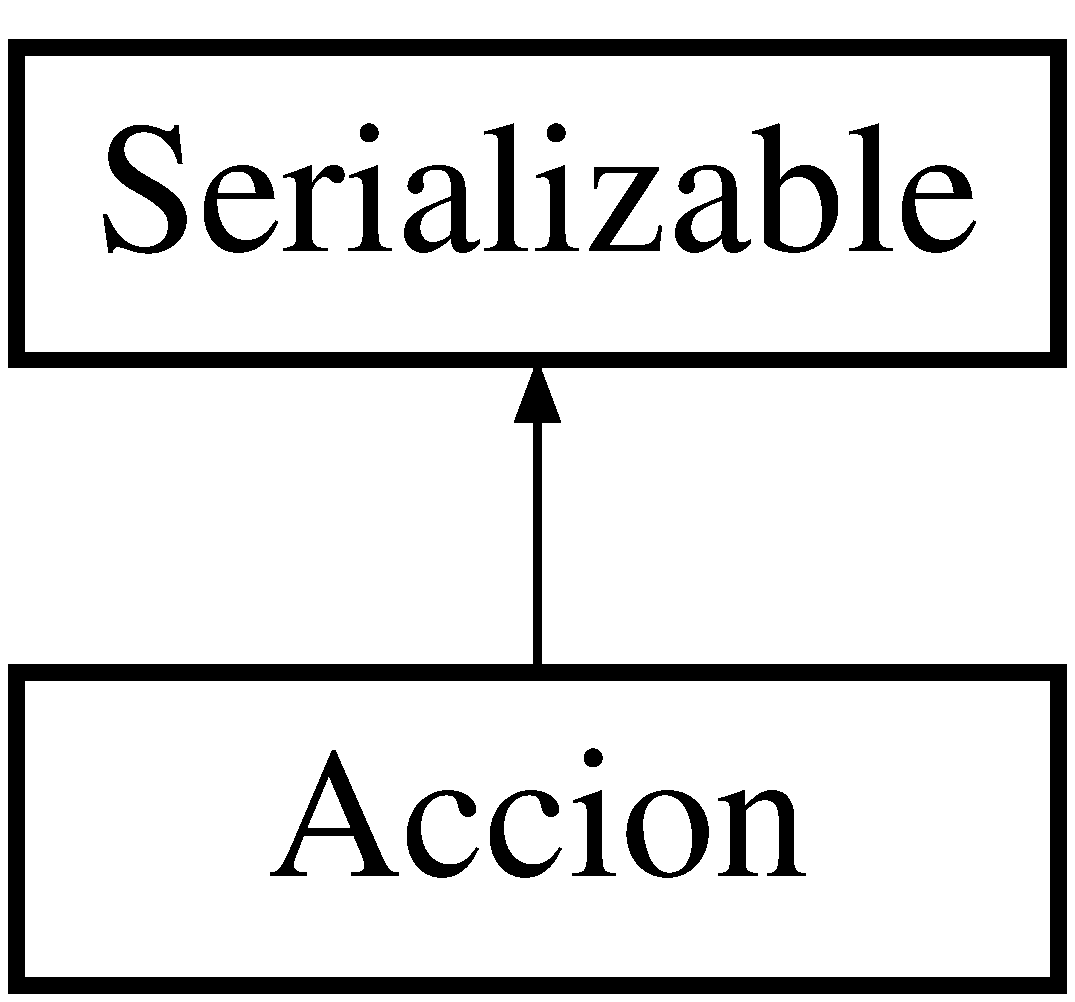
\includegraphics[height=2.000000cm]{classAccion}
\end{center}
\end{figure}
\subsection*{Public Member Functions}
\begin{DoxyCompactItemize}
\item 
String \hyperlink{classAccion_afbfc4ab0e3d6afe55075d7eb208c3a60}{get\+Nombre} ()
\begin{DoxyCompactList}\small\item\em Devuelve el nombre de la Acción. \end{DoxyCompactList}\item 
\hyperlink{classTrabajo}{Trabajo} \hyperlink{classAccion_ab299d4aa106c451865e68625ee9a2fa0}{get\+Trabajo} ()
\begin{DoxyCompactList}\small\item\em Devuelve el nombre del trabajo. \end{DoxyCompactList}\end{DoxyCompactItemize}
\subsection*{Static Public Attributes}
\begin{DoxyCompactItemize}
\item 
static final String \hyperlink{classAccion_ad8679a8a5a559e0b470231fc4c98147b}{P\+E\+D\+I\+R\+\_\+\+T\+R\+A\+B\+A\+JO} = \char`\"{}pedir\+\_\+trabajo\char`\"{}
\item 
static final String \hyperlink{classAccion_a41ff7a23c839af375260089e58ce9147}{E\+N\+V\+I\+A\+R\+\_\+\+T\+R\+A\+B\+A\+JO} = \char`\"{}enviar\+\_\+trabajo\char`\"{}
\item 
static final String \hyperlink{classAccion_a21c4e74abea5d8e84d961913979d0389}{E\+N\+V\+I\+A\+R\+\_\+\+T\+R\+A\+B\+A\+J\+O\+\_\+\+T\+E\+R\+M\+I\+N\+A\+DO} = \char`\"{}enviar\+\_\+trabajo\+\_\+terminado\char`\"{}
\item 
static final String \hyperlink{classAccion_a8c4e3447d220ea6ef7d29799f7ef2024}{F\+I\+N\+A\+L\+I\+Z\+A\+R\+\_\+\+C\+L\+I\+E\+N\+TE} = \char`\"{}finalizar\+\_\+cliente\char`\"{}
\end{DoxyCompactItemize}


\subsection{Detailed Description}
Clase que se utiliza para enviar los objetos entre servidor-\/cliente. 

\begin{DoxyAuthor}{Author}
marmol 
\end{DoxyAuthor}


\subsection{Member Function Documentation}
\index{Accion@{Accion}!get\+Nombre@{get\+Nombre}}
\index{get\+Nombre@{get\+Nombre}!Accion@{Accion}}
\subsubsection[{\texorpdfstring{get\+Nombre()}{getNombre()}}]{\setlength{\rightskip}{0pt plus 5cm}String Accion.\+get\+Nombre (
\begin{DoxyParamCaption}
{}
\end{DoxyParamCaption}
)}\hypertarget{classAccion_afbfc4ab0e3d6afe55075d7eb208c3a60}{}\label{classAccion_afbfc4ab0e3d6afe55075d7eb208c3a60}


Devuelve el nombre de la Acción. 

\begin{DoxyReturn}{Returns}

\end{DoxyReturn}
\index{Accion@{Accion}!get\+Trabajo@{get\+Trabajo}}
\index{get\+Trabajo@{get\+Trabajo}!Accion@{Accion}}
\subsubsection[{\texorpdfstring{get\+Trabajo()}{getTrabajo()}}]{\setlength{\rightskip}{0pt plus 5cm}{\bf Trabajo} Accion.\+get\+Trabajo (
\begin{DoxyParamCaption}
{}
\end{DoxyParamCaption}
)}\hypertarget{classAccion_ab299d4aa106c451865e68625ee9a2fa0}{}\label{classAccion_ab299d4aa106c451865e68625ee9a2fa0}


Devuelve el nombre del trabajo. 

\begin{DoxyReturn}{Returns}

\end{DoxyReturn}


\subsection{Member Data Documentation}
\index{Accion@{Accion}!E\+N\+V\+I\+A\+R\+\_\+\+T\+R\+A\+B\+A\+JO@{E\+N\+V\+I\+A\+R\+\_\+\+T\+R\+A\+B\+A\+JO}}
\index{E\+N\+V\+I\+A\+R\+\_\+\+T\+R\+A\+B\+A\+JO@{E\+N\+V\+I\+A\+R\+\_\+\+T\+R\+A\+B\+A\+JO}!Accion@{Accion}}
\subsubsection[{\texorpdfstring{E\+N\+V\+I\+A\+R\+\_\+\+T\+R\+A\+B\+A\+JO}{ENVIAR_TRABAJO}}]{\setlength{\rightskip}{0pt plus 5cm}final String Accion.\+E\+N\+V\+I\+A\+R\+\_\+\+T\+R\+A\+B\+A\+JO = \char`\"{}enviar\+\_\+trabajo\char`\"{}\hspace{0.3cm}{\ttfamily [static]}}\hypertarget{classAccion_a41ff7a23c839af375260089e58ce9147}{}\label{classAccion_a41ff7a23c839af375260089e58ce9147}
\index{Accion@{Accion}!E\+N\+V\+I\+A\+R\+\_\+\+T\+R\+A\+B\+A\+J\+O\+\_\+\+T\+E\+R\+M\+I\+N\+A\+DO@{E\+N\+V\+I\+A\+R\+\_\+\+T\+R\+A\+B\+A\+J\+O\+\_\+\+T\+E\+R\+M\+I\+N\+A\+DO}}
\index{E\+N\+V\+I\+A\+R\+\_\+\+T\+R\+A\+B\+A\+J\+O\+\_\+\+T\+E\+R\+M\+I\+N\+A\+DO@{E\+N\+V\+I\+A\+R\+\_\+\+T\+R\+A\+B\+A\+J\+O\+\_\+\+T\+E\+R\+M\+I\+N\+A\+DO}!Accion@{Accion}}
\subsubsection[{\texorpdfstring{E\+N\+V\+I\+A\+R\+\_\+\+T\+R\+A\+B\+A\+J\+O\+\_\+\+T\+E\+R\+M\+I\+N\+A\+DO}{ENVIAR_TRABAJO_TERMINADO}}]{\setlength{\rightskip}{0pt plus 5cm}final String Accion.\+E\+N\+V\+I\+A\+R\+\_\+\+T\+R\+A\+B\+A\+J\+O\+\_\+\+T\+E\+R\+M\+I\+N\+A\+DO = \char`\"{}enviar\+\_\+trabajo\+\_\+terminado\char`\"{}\hspace{0.3cm}{\ttfamily [static]}}\hypertarget{classAccion_a21c4e74abea5d8e84d961913979d0389}{}\label{classAccion_a21c4e74abea5d8e84d961913979d0389}
\index{Accion@{Accion}!F\+I\+N\+A\+L\+I\+Z\+A\+R\+\_\+\+C\+L\+I\+E\+N\+TE@{F\+I\+N\+A\+L\+I\+Z\+A\+R\+\_\+\+C\+L\+I\+E\+N\+TE}}
\index{F\+I\+N\+A\+L\+I\+Z\+A\+R\+\_\+\+C\+L\+I\+E\+N\+TE@{F\+I\+N\+A\+L\+I\+Z\+A\+R\+\_\+\+C\+L\+I\+E\+N\+TE}!Accion@{Accion}}
\subsubsection[{\texorpdfstring{F\+I\+N\+A\+L\+I\+Z\+A\+R\+\_\+\+C\+L\+I\+E\+N\+TE}{FINALIZAR_CLIENTE}}]{\setlength{\rightskip}{0pt plus 5cm}final String Accion.\+F\+I\+N\+A\+L\+I\+Z\+A\+R\+\_\+\+C\+L\+I\+E\+N\+TE = \char`\"{}finalizar\+\_\+cliente\char`\"{}\hspace{0.3cm}{\ttfamily [static]}}\hypertarget{classAccion_a8c4e3447d220ea6ef7d29799f7ef2024}{}\label{classAccion_a8c4e3447d220ea6ef7d29799f7ef2024}
\index{Accion@{Accion}!P\+E\+D\+I\+R\+\_\+\+T\+R\+A\+B\+A\+JO@{P\+E\+D\+I\+R\+\_\+\+T\+R\+A\+B\+A\+JO}}
\index{P\+E\+D\+I\+R\+\_\+\+T\+R\+A\+B\+A\+JO@{P\+E\+D\+I\+R\+\_\+\+T\+R\+A\+B\+A\+JO}!Accion@{Accion}}
\subsubsection[{\texorpdfstring{P\+E\+D\+I\+R\+\_\+\+T\+R\+A\+B\+A\+JO}{PEDIR_TRABAJO}}]{\setlength{\rightskip}{0pt plus 5cm}final String Accion.\+P\+E\+D\+I\+R\+\_\+\+T\+R\+A\+B\+A\+JO = \char`\"{}pedir\+\_\+trabajo\char`\"{}\hspace{0.3cm}{\ttfamily [static]}}\hypertarget{classAccion_ad8679a8a5a559e0b470231fc4c98147b}{}\label{classAccion_ad8679a8a5a559e0b470231fc4c98147b}


The documentation for this class was generated from the following file\+:\begin{DoxyCompactItemize}
\item 
src/\hyperlink{Accion_8java}{Accion.\+java}\end{DoxyCompactItemize}

\hypertarget{classCliente}{}\section{Cliente Class Reference}
\label{classCliente}\index{Cliente@{Cliente}}


Implementa la conexión individual con el \hyperlink{classServidor}{Servidor} y realiza las acciones oportunas con los objetos \hyperlink{classTrabajo}{Trabajo}.  


Inheritance diagram for Cliente\+:\begin{figure}[H]
\begin{center}
\leavevmode
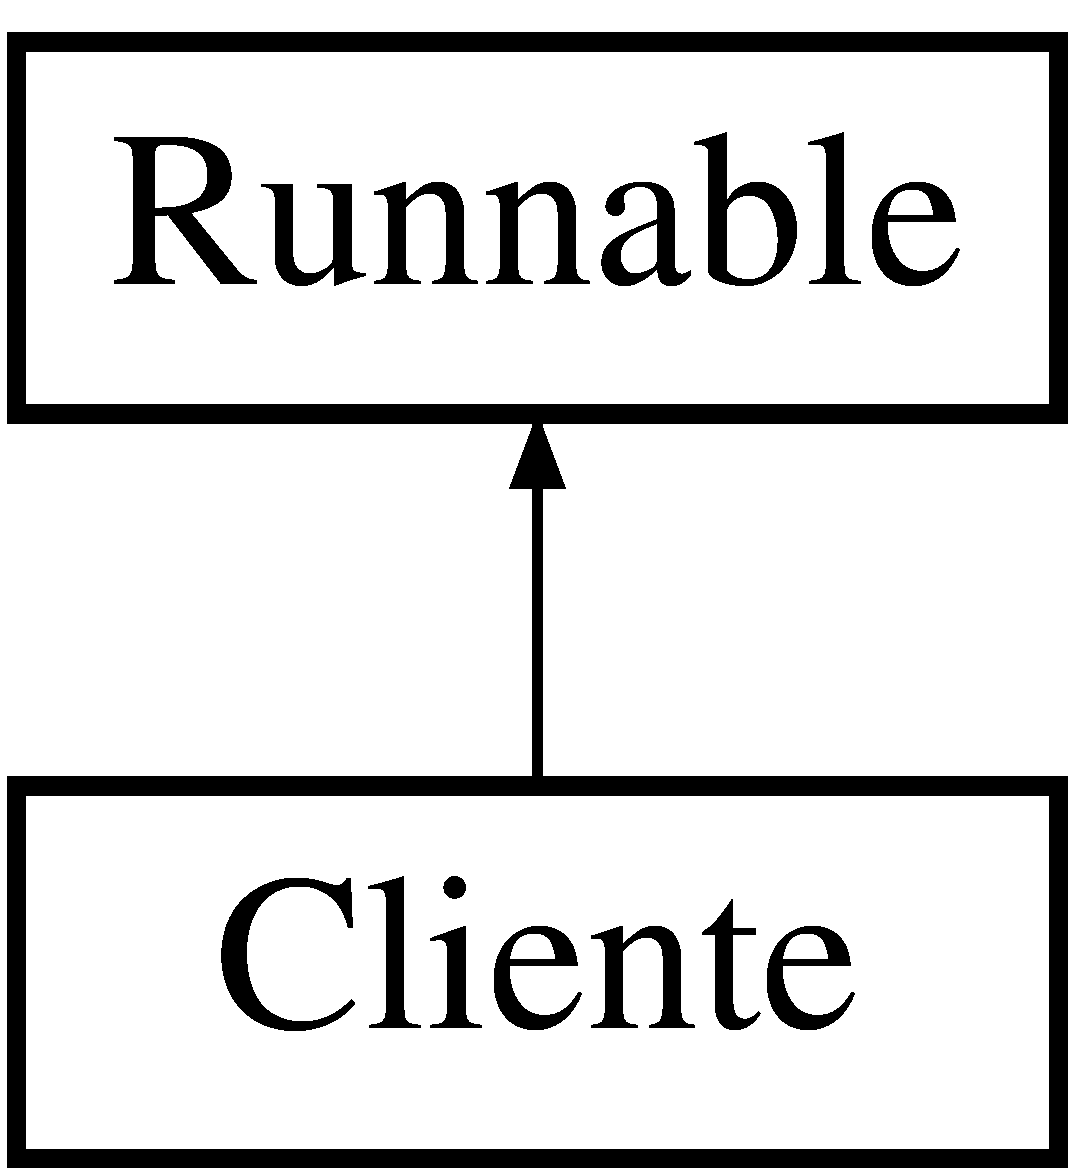
\includegraphics[height=2.000000cm]{classCliente}
\end{center}
\end{figure}
\subsection*{Public Member Functions}
\begin{DoxyCompactItemize}
\item 
void \hyperlink{classCliente_a18bd3f9c4d4006b311fd226ca5336dda}{run} ()
\begin{DoxyCompactList}\small\item\em Códigod el Thread. \end{DoxyCompactList}\end{DoxyCompactItemize}
\subsection*{Static Public Member Functions}
\begin{DoxyCompactItemize}
\item 
static void \hyperlink{classCliente_a221cda5443459d5da734d24d3b789ac0}{main} (String\mbox{[}$\,$\mbox{]} args)
\begin{DoxyCompactList}\small\item\em Programa principal de los clientes Crea tantos clientes como se especifique y se conectan al servidor. \end{DoxyCompactList}\end{DoxyCompactItemize}
\subsection*{Static Public Attributes}
\begin{DoxyCompactItemize}
\item 
static final int \hyperlink{classCliente_a48a0a2f19643c23979a654493e344bbb}{N\+U\+M\+E\+R\+O\+\_\+\+C\+L\+I\+E\+N\+T\+ES} = 16
\end{DoxyCompactItemize}


\subsection{Detailed Description}
Implementa la conexión individual con el \hyperlink{classServidor}{Servidor} y realiza las acciones oportunas con los objetos \hyperlink{classTrabajo}{Trabajo}. 

\begin{DoxyAuthor}{Author}
marmol 
\end{DoxyAuthor}


\subsection{Member Function Documentation}
\index{Cliente@{Cliente}!main@{main}}
\index{main@{main}!Cliente@{Cliente}}
\subsubsection[{\texorpdfstring{main(\+String[] args)}{main(String[] args)}}]{\setlength{\rightskip}{0pt plus 5cm}static void Cliente.\+main (
\begin{DoxyParamCaption}
\item[{String\mbox{[}$\,$\mbox{]}}]{args}
\end{DoxyParamCaption}
)\hspace{0.3cm}{\ttfamily [static]}}\hypertarget{classCliente_a221cda5443459d5da734d24d3b789ac0}{}\label{classCliente_a221cda5443459d5da734d24d3b789ac0}


Programa principal de los clientes Crea tantos clientes como se especifique y se conectan al servidor. 


\begin{DoxyParams}{Parameters}
{\em args} & Un vector con\+: hostname puerto \mbox{[}n\+Clientes\mbox{]} \\
\hline
\end{DoxyParams}
\index{Cliente@{Cliente}!run@{run}}
\index{run@{run}!Cliente@{Cliente}}
\subsubsection[{\texorpdfstring{run()}{run()}}]{\setlength{\rightskip}{0pt plus 5cm}void Cliente.\+run (
\begin{DoxyParamCaption}
{}
\end{DoxyParamCaption}
)}\hypertarget{classCliente_a18bd3f9c4d4006b311fd226ca5336dda}{}\label{classCliente_a18bd3f9c4d4006b311fd226ca5336dda}


Códigod el Thread. 



\subsection{Member Data Documentation}
\index{Cliente@{Cliente}!N\+U\+M\+E\+R\+O\+\_\+\+C\+L\+I\+E\+N\+T\+ES@{N\+U\+M\+E\+R\+O\+\_\+\+C\+L\+I\+E\+N\+T\+ES}}
\index{N\+U\+M\+E\+R\+O\+\_\+\+C\+L\+I\+E\+N\+T\+ES@{N\+U\+M\+E\+R\+O\+\_\+\+C\+L\+I\+E\+N\+T\+ES}!Cliente@{Cliente}}
\subsubsection[{\texorpdfstring{N\+U\+M\+E\+R\+O\+\_\+\+C\+L\+I\+E\+N\+T\+ES}{NUMERO_CLIENTES}}]{\setlength{\rightskip}{0pt plus 5cm}final int Cliente.\+N\+U\+M\+E\+R\+O\+\_\+\+C\+L\+I\+E\+N\+T\+ES = 16\hspace{0.3cm}{\ttfamily [static]}}\hypertarget{classCliente_a48a0a2f19643c23979a654493e344bbb}{}\label{classCliente_a48a0a2f19643c23979a654493e344bbb}


The documentation for this class was generated from the following file\+:\begin{DoxyCompactItemize}
\item 
src/\hyperlink{Cliente_8java}{Cliente.\+java}\end{DoxyCompactItemize}

\hypertarget{classMandelbrot}{}\section{Mandelbrot Class Reference}
\label{classMandelbrot}\index{Mandelbrot@{Mandelbrot}}


Implementa el método necesario para crear un conjunto de \hyperlink{classMandelbrot}{Mandelbrot}.  


\subsection*{Static Public Member Functions}
\begin{DoxyCompactItemize}
\item 
static void \hyperlink{classMandelbrot_a50f066c6f668f81af310aed0a18f6615}{realizar\+Trabajo} (\hyperlink{classTrabajo}{Trabajo} trabajo)
\begin{DoxyCompactList}\small\item\em Procesa un conjunto de \hyperlink{classMandelbrot}{Mandelbrot} en base a unos argumentos recibidos en un \hyperlink{classTrabajo}{Trabajo}. \end{DoxyCompactList}\end{DoxyCompactItemize}


\subsection{Detailed Description}
Implementa el método necesario para crear un conjunto de \hyperlink{classMandelbrot}{Mandelbrot}. 

\begin{DoxyAuthor}{Author}
marmol 
\end{DoxyAuthor}


\subsection{Member Function Documentation}
\index{Mandelbrot@{Mandelbrot}!realizar\+Trabajo@{realizar\+Trabajo}}
\index{realizar\+Trabajo@{realizar\+Trabajo}!Mandelbrot@{Mandelbrot}}
\subsubsection[{\texorpdfstring{realizar\+Trabajo(\+Trabajo trabajo)}{realizarTrabajo(Trabajo trabajo)}}]{\setlength{\rightskip}{0pt plus 5cm}static void Mandelbrot.\+realizar\+Trabajo (
\begin{DoxyParamCaption}
\item[{{\bf Trabajo}}]{trabajo}
\end{DoxyParamCaption}
)\hspace{0.3cm}{\ttfamily [static]}}\hypertarget{classMandelbrot_a50f066c6f668f81af310aed0a18f6615}{}\label{classMandelbrot_a50f066c6f668f81af310aed0a18f6615}


Procesa un conjunto de \hyperlink{classMandelbrot}{Mandelbrot} en base a unos argumentos recibidos en un \hyperlink{classTrabajo}{Trabajo}. 


\begin{DoxyParams}{Parameters}
{\em trabajo} & Contiene los argumentos necesarios para procesar el conjunto de \hyperlink{classMandelbrot}{Mandelbrot}. Provee de una estructura para guardar los cambios. \\
\hline
\end{DoxyParams}


The documentation for this class was generated from the following file\+:\begin{DoxyCompactItemize}
\item 
src/\hyperlink{Mandelbrot_8java}{Mandelbrot.\+java}\end{DoxyCompactItemize}

\hypertarget{classPGM}{}\section{P\+GM Class Reference}
\label{classPGM}\index{P\+GM@{P\+GM}}


Implementa el tratamiento de archivos \hyperlink{classPGM}{P\+GM} a partir de matrices de Color.  


\subsection*{Public Member Functions}
\begin{DoxyCompactItemize}
\item 
void \hyperlink{classPGM_ab02ef4437d19725dbd8cf7f183c243e9}{anhadir} (Color\mbox{[}$\,$\mbox{]}\mbox{[}$\,$\mbox{]} content)  throws I\+O\+Exception
\begin{DoxyCompactList}\small\item\em Añade una matriz de Color a la imagen. \end{DoxyCompactList}\item 
void \hyperlink{classPGM_abef1cc9459a0efcf719b52dc5d4670cf}{cerrar} ()  throws I\+O\+Exception 
\begin{DoxyCompactList}\small\item\em Cierra el archivo cuando se finalizan las operaciones. \end{DoxyCompactList}\end{DoxyCompactItemize}


\subsection{Detailed Description}
Implementa el tratamiento de archivos \hyperlink{classPGM}{P\+GM} a partir de matrices de Color. 

\begin{DoxyAuthor}{Author}
marmol 
\end{DoxyAuthor}


\subsection{Member Function Documentation}
\index{P\+GM@{P\+GM}!anhadir@{anhadir}}
\index{anhadir@{anhadir}!P\+GM@{P\+GM}}
\subsubsection[{\texorpdfstring{anhadir(\+Color[][] content)}{anhadir(Color[][] content)}}]{\setlength{\rightskip}{0pt plus 5cm}void P\+G\+M.\+anhadir (
\begin{DoxyParamCaption}
\item[{Color}]{content\mbox{[}$\,$\mbox{]}\mbox{[}$\,$\mbox{]}}
\end{DoxyParamCaption}
) throws I\+O\+Exception}\hypertarget{classPGM_ab02ef4437d19725dbd8cf7f183c243e9}{}\label{classPGM_ab02ef4437d19725dbd8cf7f183c243e9}


Añade una matriz de Color a la imagen. 


\begin{DoxyParams}{Parameters}
{\em content} & La matriz los colores \\
\hline
\end{DoxyParams}

\begin{DoxyExceptions}{Exceptions}
{\em I\+O\+Exception} & \\
\hline
\end{DoxyExceptions}
\index{P\+GM@{P\+GM}!cerrar@{cerrar}}
\index{cerrar@{cerrar}!P\+GM@{P\+GM}}
\subsubsection[{\texorpdfstring{cerrar()}{cerrar()}}]{\setlength{\rightskip}{0pt plus 5cm}void P\+G\+M.\+cerrar (
\begin{DoxyParamCaption}
{}
\end{DoxyParamCaption}
) throws I\+O\+Exception}\hypertarget{classPGM_abef1cc9459a0efcf719b52dc5d4670cf}{}\label{classPGM_abef1cc9459a0efcf719b52dc5d4670cf}


Cierra el archivo cuando se finalizan las operaciones. 


\begin{DoxyExceptions}{Exceptions}
{\em I\+O\+Exception} & \\
\hline
\end{DoxyExceptions}


The documentation for this class was generated from the following file\+:\begin{DoxyCompactItemize}
\item 
src/\hyperlink{PGM_8java}{P\+G\+M.\+java}\end{DoxyCompactItemize}

\hypertarget{classServidor}{}\section{Servidor Class Reference}
\label{classServidor}\index{Servidor@{Servidor}}


Implementa la clase \hyperlink{classServidor}{Servidor} que gestiona todas las conexiones y los trabajos.  


Inheritance diagram for Servidor\+:\begin{figure}[H]
\begin{center}
\leavevmode
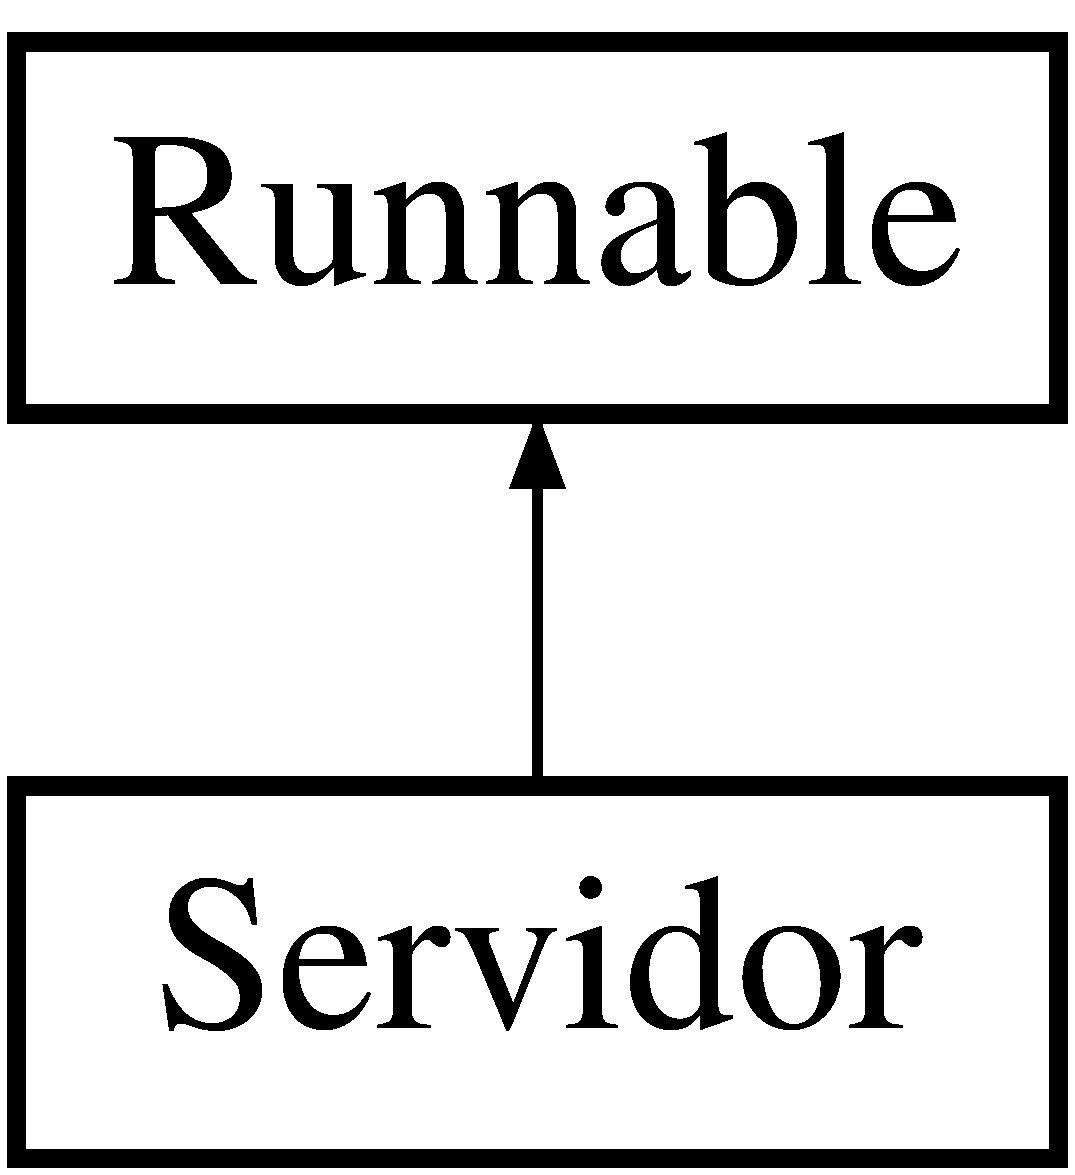
\includegraphics[height=2.000000cm]{classServidor}
\end{center}
\end{figure}
\subsection*{Public Member Functions}
\begin{DoxyCompactItemize}
\item 
synchronized boolean \hyperlink{classServidor_a210f62b0f4ccd1d3eccc6eff7051d640}{estan\+Trabajos\+Completados} ()
\begin{DoxyCompactList}\small\item\em Comprueba si los trabajos estan completados. \end{DoxyCompactList}\item 
synchronized boolean \hyperlink{classServidor_ad2d3e79eeac3e52edcec0c4ef17ffce6}{hay\+Trabajos\+Por\+Realizar} ()
\begin{DoxyCompactList}\small\item\em Comprueba si hay trabajos por realizar. \end{DoxyCompactList}\item 
synchronized \hyperlink{classTrabajo}{Trabajo} \hyperlink{classServidor_a1afa144ebeacbf0e9960ab8b5a1d3419}{sacar\+Trabajo\+Sin\+Realizar} ()
\begin{DoxyCompactList}\small\item\em Saca un trabajo sin realizar, lo mete en realizando y devuelve el \hyperlink{classTrabajo}{Trabajo}. \end{DoxyCompactList}\item 
synchronized void \hyperlink{classServidor_a94e88d197276e470cb7373b8ca3ae847}{anhadir\+Trabajo\+Realizado} (\hyperlink{classTrabajo}{Trabajo} t)  throws Exception 
\begin{DoxyCompactList}\small\item\em Añade un trabajo que estaba siendo realizado y ahora esa completado (procesado) por un \hyperlink{classCliente}{Cliente}. \end{DoxyCompactList}\item 
synchronized void \hyperlink{classServidor_a15c19b2947826047e0664915f86a16d8}{devolver\+Trabajo\+Realizando} (\hyperlink{classTrabajo}{Trabajo} t)
\begin{DoxyCompactList}\small\item\em Devuelve un trabajo que estaba siendo realizado pero que no pudo ser completado (error en \hyperlink{classCliente}{Cliente}) \end{DoxyCompactList}\item 
void \hyperlink{classServidor_adc224162ae15224464bf33d0f6bf79e9}{esperar\+Cambios\+Trabajos\+Realizando} ()
\begin{DoxyCompactList}\small\item\em Duerme un proceso hasta que se produzcan cambios los trabajos que se están realizando. \end{DoxyCompactList}\item 
void \hyperlink{classServidor_a7dcc9a8eaf0ab0e7eedd0fb41c03849c}{notificar\+Cambios\+Trabajos\+Realizando} ()
\begin{DoxyCompactList}\small\item\em Notifica que se han producido cambios en los trabajos que se están realizando. \end{DoxyCompactList}\item 
synchronized void \hyperlink{classServidor_a6dda49cac122c1933278bae21641bff4}{finalizar} ()  throws Unknown\+Host\+Exception, I\+O\+Exception 
\begin{DoxyCompactList}\small\item\em Notifica que todos los trabajos se finalizaron. \end{DoxyCompactList}\item 
void \hyperlink{classServidor_a24622869d200039d3e0df70b6e29eb9e}{run} ()
\begin{DoxyCompactList}\small\item\em Gestiona las conexiones entrantes no se acaben los trabajos. \end{DoxyCompactList}\end{DoxyCompactItemize}
\subsection*{Static Public Member Functions}
\begin{DoxyCompactItemize}
\item 
static void \hyperlink{classServidor_a4f1d3d541947003e9c4db0b0ad40bd1d}{main} (String\mbox{[}$\,$\mbox{]} args)
\begin{DoxyCompactList}\small\item\em Programa \hyperlink{classServidor}{Servidor} principal. \end{DoxyCompactList}\end{DoxyCompactItemize}


\subsection{Detailed Description}
Implementa la clase \hyperlink{classServidor}{Servidor} que gestiona todas las conexiones y los trabajos. 

\begin{DoxyAuthor}{Author}
marmol 
\end{DoxyAuthor}


\subsection{Member Function Documentation}
\index{Servidor@{Servidor}!anhadir\+Trabajo\+Realizado@{anhadir\+Trabajo\+Realizado}}
\index{anhadir\+Trabajo\+Realizado@{anhadir\+Trabajo\+Realizado}!Servidor@{Servidor}}
\subsubsection[{\texorpdfstring{anhadir\+Trabajo\+Realizado(\+Trabajo t)}{anhadirTrabajoRealizado(Trabajo t)}}]{\setlength{\rightskip}{0pt plus 5cm}synchronized void Servidor.\+anhadir\+Trabajo\+Realizado (
\begin{DoxyParamCaption}
\item[{{\bf Trabajo}}]{t}
\end{DoxyParamCaption}
) throws Exception}\hypertarget{classServidor_a94e88d197276e470cb7373b8ca3ae847}{}\label{classServidor_a94e88d197276e470cb7373b8ca3ae847}


Añade un trabajo que estaba siendo realizado y ahora esa completado (procesado) por un \hyperlink{classCliente}{Cliente}. 


\begin{DoxyParams}{Parameters}
{\em t} & El trabajo \\
\hline
\end{DoxyParams}

\begin{DoxyExceptions}{Exceptions}
{\em Exception} & \\
\hline
\end{DoxyExceptions}
\index{Servidor@{Servidor}!devolver\+Trabajo\+Realizando@{devolver\+Trabajo\+Realizando}}
\index{devolver\+Trabajo\+Realizando@{devolver\+Trabajo\+Realizando}!Servidor@{Servidor}}
\subsubsection[{\texorpdfstring{devolver\+Trabajo\+Realizando(\+Trabajo t)}{devolverTrabajoRealizando(Trabajo t)}}]{\setlength{\rightskip}{0pt plus 5cm}synchronized void Servidor.\+devolver\+Trabajo\+Realizando (
\begin{DoxyParamCaption}
\item[{{\bf Trabajo}}]{t}
\end{DoxyParamCaption}
)}\hypertarget{classServidor_a15c19b2947826047e0664915f86a16d8}{}\label{classServidor_a15c19b2947826047e0664915f86a16d8}


Devuelve un trabajo que estaba siendo realizado pero que no pudo ser completado (error en \hyperlink{classCliente}{Cliente}) 


\begin{DoxyParams}{Parameters}
{\em t} & El trabajo \\
\hline
\end{DoxyParams}
\index{Servidor@{Servidor}!esperar\+Cambios\+Trabajos\+Realizando@{esperar\+Cambios\+Trabajos\+Realizando}}
\index{esperar\+Cambios\+Trabajos\+Realizando@{esperar\+Cambios\+Trabajos\+Realizando}!Servidor@{Servidor}}
\subsubsection[{\texorpdfstring{esperar\+Cambios\+Trabajos\+Realizando()}{esperarCambiosTrabajosRealizando()}}]{\setlength{\rightskip}{0pt plus 5cm}void Servidor.\+esperar\+Cambios\+Trabajos\+Realizando (
\begin{DoxyParamCaption}
{}
\end{DoxyParamCaption}
)}\hypertarget{classServidor_adc224162ae15224464bf33d0f6bf79e9}{}\label{classServidor_adc224162ae15224464bf33d0f6bf79e9}


Duerme un proceso hasta que se produzcan cambios los trabajos que se están realizando. 

\index{Servidor@{Servidor}!estan\+Trabajos\+Completados@{estan\+Trabajos\+Completados}}
\index{estan\+Trabajos\+Completados@{estan\+Trabajos\+Completados}!Servidor@{Servidor}}
\subsubsection[{\texorpdfstring{estan\+Trabajos\+Completados()}{estanTrabajosCompletados()}}]{\setlength{\rightskip}{0pt plus 5cm}synchronized boolean Servidor.\+estan\+Trabajos\+Completados (
\begin{DoxyParamCaption}
{}
\end{DoxyParamCaption}
)}\hypertarget{classServidor_a210f62b0f4ccd1d3eccc6eff7051d640}{}\label{classServidor_a210f62b0f4ccd1d3eccc6eff7051d640}


Comprueba si los trabajos estan completados. 

\begin{DoxyReturn}{Returns}

\end{DoxyReturn}
\index{Servidor@{Servidor}!finalizar@{finalizar}}
\index{finalizar@{finalizar}!Servidor@{Servidor}}
\subsubsection[{\texorpdfstring{finalizar()}{finalizar()}}]{\setlength{\rightskip}{0pt plus 5cm}synchronized void Servidor.\+finalizar (
\begin{DoxyParamCaption}
{}
\end{DoxyParamCaption}
) throws Unknown\+Host\+Exception, I\+O\+Exception}\hypertarget{classServidor_a6dda49cac122c1933278bae21641bff4}{}\label{classServidor_a6dda49cac122c1933278bae21641bff4}


Notifica que todos los trabajos se finalizaron. 


\begin{DoxyExceptions}{Exceptions}
{\em Unknown\+Host\+Exception} & \\
\hline
{\em I\+O\+Exception} & \\
\hline
\end{DoxyExceptions}
\index{Servidor@{Servidor}!hay\+Trabajos\+Por\+Realizar@{hay\+Trabajos\+Por\+Realizar}}
\index{hay\+Trabajos\+Por\+Realizar@{hay\+Trabajos\+Por\+Realizar}!Servidor@{Servidor}}
\subsubsection[{\texorpdfstring{hay\+Trabajos\+Por\+Realizar()}{hayTrabajosPorRealizar()}}]{\setlength{\rightskip}{0pt plus 5cm}synchronized boolean Servidor.\+hay\+Trabajos\+Por\+Realizar (
\begin{DoxyParamCaption}
{}
\end{DoxyParamCaption}
)}\hypertarget{classServidor_ad2d3e79eeac3e52edcec0c4ef17ffce6}{}\label{classServidor_ad2d3e79eeac3e52edcec0c4ef17ffce6}


Comprueba si hay trabajos por realizar. 

\begin{DoxyReturn}{Returns}

\end{DoxyReturn}
\index{Servidor@{Servidor}!main@{main}}
\index{main@{main}!Servidor@{Servidor}}
\subsubsection[{\texorpdfstring{main(\+String[] args)}{main(String[] args)}}]{\setlength{\rightskip}{0pt plus 5cm}static void Servidor.\+main (
\begin{DoxyParamCaption}
\item[{String\mbox{[}$\,$\mbox{]}}]{args}
\end{DoxyParamCaption}
)\hspace{0.3cm}{\ttfamily [static]}}\hypertarget{classServidor_a4f1d3d541947003e9c4db0b0ad40bd1d}{}\label{classServidor_a4f1d3d541947003e9c4db0b0ad40bd1d}


Programa \hyperlink{classServidor}{Servidor} principal. 


\begin{DoxyParams}{Parameters}
{\em args} & Argumentos\+: puerto divisiones x\+Centro y\+Centro tamaño iteraciones archivo \\
\hline
\end{DoxyParams}
\index{Servidor@{Servidor}!notificar\+Cambios\+Trabajos\+Realizando@{notificar\+Cambios\+Trabajos\+Realizando}}
\index{notificar\+Cambios\+Trabajos\+Realizando@{notificar\+Cambios\+Trabajos\+Realizando}!Servidor@{Servidor}}
\subsubsection[{\texorpdfstring{notificar\+Cambios\+Trabajos\+Realizando()}{notificarCambiosTrabajosRealizando()}}]{\setlength{\rightskip}{0pt plus 5cm}void Servidor.\+notificar\+Cambios\+Trabajos\+Realizando (
\begin{DoxyParamCaption}
{}
\end{DoxyParamCaption}
)}\hypertarget{classServidor_a7dcc9a8eaf0ab0e7eedd0fb41c03849c}{}\label{classServidor_a7dcc9a8eaf0ab0e7eedd0fb41c03849c}


Notifica que se han producido cambios en los trabajos que se están realizando. 

\index{Servidor@{Servidor}!run@{run}}
\index{run@{run}!Servidor@{Servidor}}
\subsubsection[{\texorpdfstring{run()}{run()}}]{\setlength{\rightskip}{0pt plus 5cm}void Servidor.\+run (
\begin{DoxyParamCaption}
{}
\end{DoxyParamCaption}
)}\hypertarget{classServidor_a24622869d200039d3e0df70b6e29eb9e}{}\label{classServidor_a24622869d200039d3e0df70b6e29eb9e}


Gestiona las conexiones entrantes no se acaben los trabajos. 

\index{Servidor@{Servidor}!sacar\+Trabajo\+Sin\+Realizar@{sacar\+Trabajo\+Sin\+Realizar}}
\index{sacar\+Trabajo\+Sin\+Realizar@{sacar\+Trabajo\+Sin\+Realizar}!Servidor@{Servidor}}
\subsubsection[{\texorpdfstring{sacar\+Trabajo\+Sin\+Realizar()}{sacarTrabajoSinRealizar()}}]{\setlength{\rightskip}{0pt plus 5cm}synchronized {\bf Trabajo} Servidor.\+sacar\+Trabajo\+Sin\+Realizar (
\begin{DoxyParamCaption}
{}
\end{DoxyParamCaption}
)}\hypertarget{classServidor_a1afa144ebeacbf0e9960ab8b5a1d3419}{}\label{classServidor_a1afa144ebeacbf0e9960ab8b5a1d3419}


Saca un trabajo sin realizar, lo mete en realizando y devuelve el \hyperlink{classTrabajo}{Trabajo}. 

\begin{DoxyReturn}{Returns}

\end{DoxyReturn}


The documentation for this class was generated from the following file\+:\begin{DoxyCompactItemize}
\item 
src/\hyperlink{Servidor_8java}{Servidor.\+java}\end{DoxyCompactItemize}

\hypertarget{classServidorThread}{}\section{Servidor\+Thread Class Reference}
\label{classServidorThread}\index{Servidor\+Thread@{Servidor\+Thread}}


Clase que se encarga de gestionar individualmente cada conexión con el cliente en el servidor.  


Inheritance diagram for Servidor\+Thread\+:\begin{figure}[H]
\begin{center}
\leavevmode
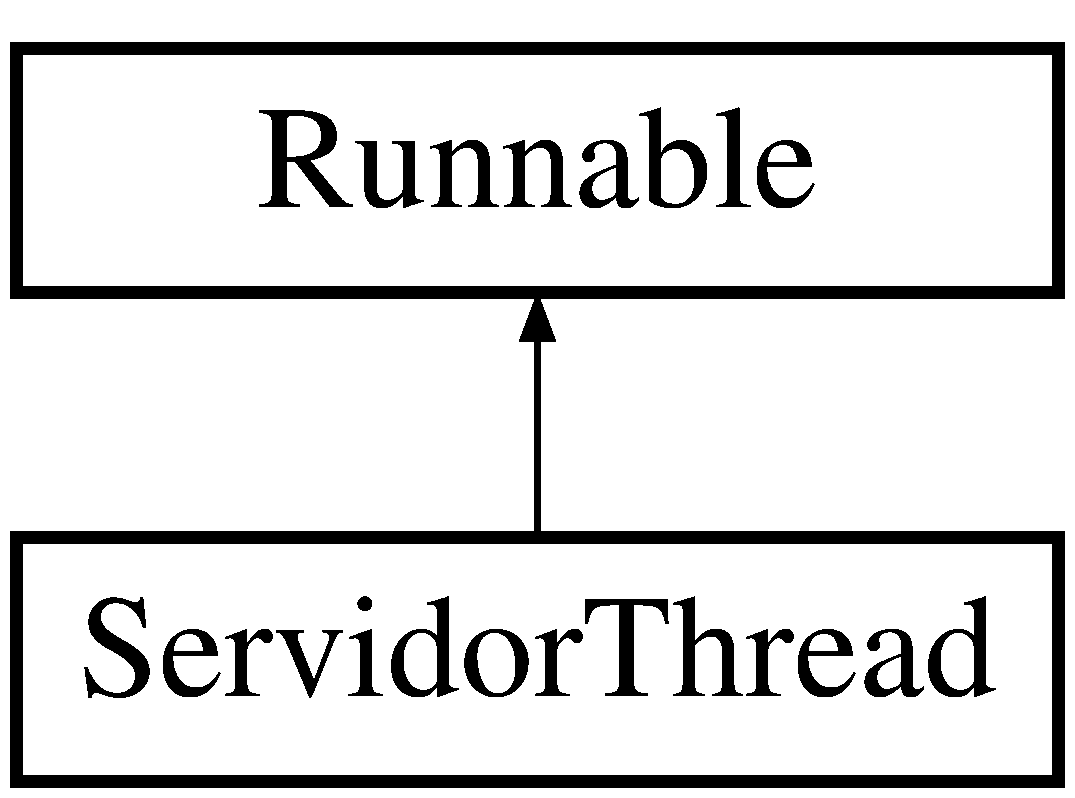
\includegraphics[height=2.000000cm]{classServidorThread}
\end{center}
\end{figure}
\subsection*{Public Member Functions}
\begin{DoxyCompactItemize}
\item 
void \hyperlink{classServidorThread_adf6d9355c8ae91c077461b5e2d569fdb}{run} ()
\begin{DoxyCompactList}\small\item\em Código del Thread que gestiona la conexión con el cliente. \end{DoxyCompactList}\end{DoxyCompactItemize}


\subsection{Detailed Description}
Clase que se encarga de gestionar individualmente cada conexión con el cliente en el servidor. 

\begin{DoxyAuthor}{Author}
marmol 
\end{DoxyAuthor}


\subsection{Member Function Documentation}
\index{Servidor\+Thread@{Servidor\+Thread}!run@{run}}
\index{run@{run}!Servidor\+Thread@{Servidor\+Thread}}
\subsubsection[{\texorpdfstring{run()}{run()}}]{\setlength{\rightskip}{0pt plus 5cm}void Servidor\+Thread.\+run (
\begin{DoxyParamCaption}
{}
\end{DoxyParamCaption}
)}\hypertarget{classServidorThread_adf6d9355c8ae91c077461b5e2d569fdb}{}\label{classServidorThread_adf6d9355c8ae91c077461b5e2d569fdb}


Código del Thread que gestiona la conexión con el cliente. 



The documentation for this class was generated from the following file\+:\begin{DoxyCompactItemize}
\item 
src/\hyperlink{ServidorThread_8java}{Servidor\+Thread.\+java}\end{DoxyCompactItemize}

\hypertarget{classTrabajo}{}\section{Trabajo Class Reference}
\label{classTrabajo}\index{Trabajo@{Trabajo}}


Contiene los argumentos necesarios para procesar el conjunto de \hyperlink{classMandelbrot}{Mandelbrot} y ofrece una estructura para guardar los resultados.  


Inheritance diagram for Trabajo\+:\begin{figure}[H]
\begin{center}
\leavevmode
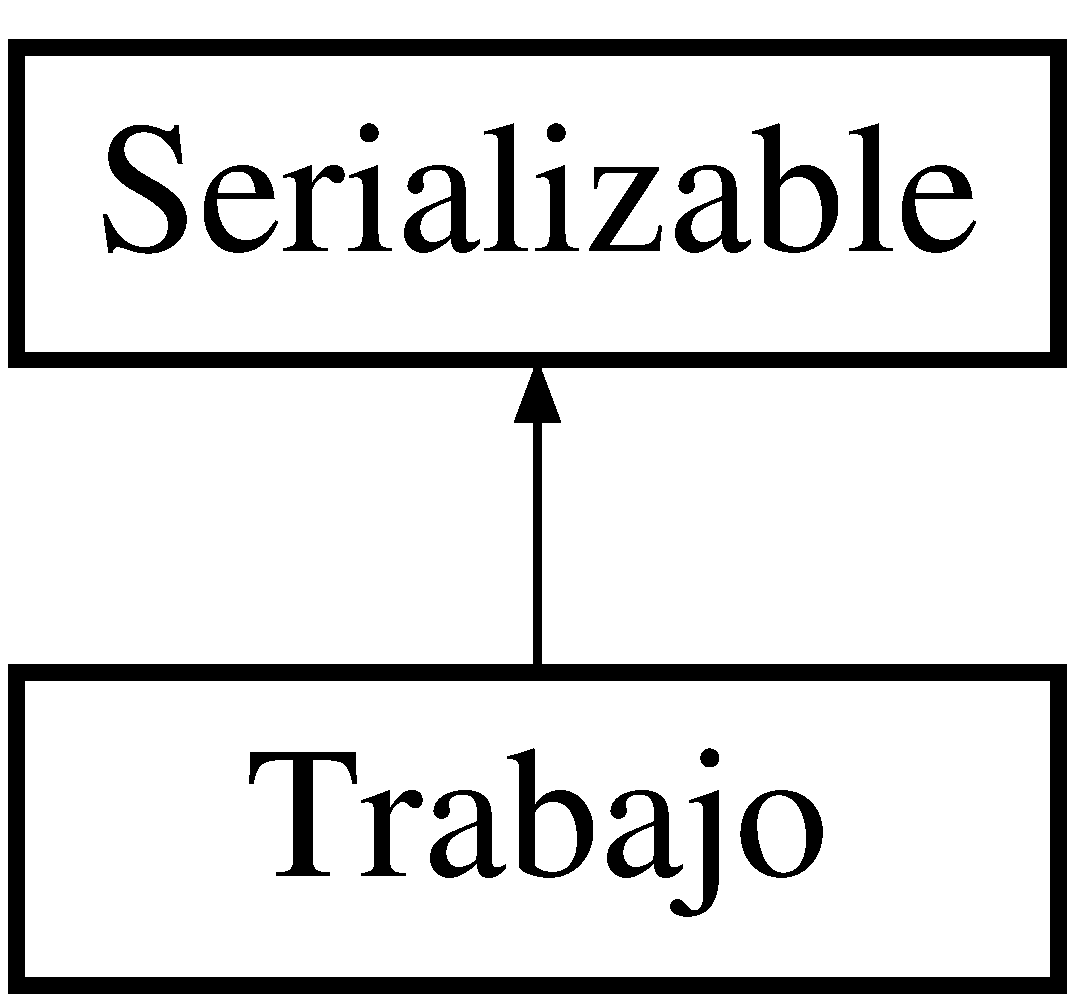
\includegraphics[height=2.000000cm]{classTrabajo}
\end{center}
\end{figure}
\subsection*{Public Member Functions}
\begin{DoxyCompactItemize}
\item 
int \hyperlink{classTrabajo_af9f14641f1998f17ae95631a8cc6859d}{get\+Posicion} ()
\begin{DoxyCompactList}\small\item\em Obtiene la posición de la zona en la imagen final. \end{DoxyCompactList}\item 
void \hyperlink{classTrabajo_ac32572a4925d6749fc46d18a056f1529}{set} (double x, double y, Color color)
\begin{DoxyCompactList}\small\item\em Establece un color de un píxel. \end{DoxyCompactList}\item 
int \hyperlink{classTrabajo_a0fe8005e31fc4e71e66fcf8cad67dc6a}{get\+XI} ()
\begin{DoxyCompactList}\small\item\em Obtiene la coordenada X del punto inicial. \end{DoxyCompactList}\item 
int \hyperlink{classTrabajo_a9b0bbf4c170c64b9e4af5444441f5487}{get\+YI} ()
\begin{DoxyCompactList}\small\item\em Obtiene la coordenada y del punto inicial. \end{DoxyCompactList}\item 
Color\mbox{[}$\,$\mbox{]}\mbox{[}$\,$\mbox{]} \hyperlink{classTrabajo_a5f807db0cb4016a3deffea7bb3b387c4}{get\+Matriz} ()
\begin{DoxyCompactList}\small\item\em Obtiene la matriz de colores. \end{DoxyCompactList}\end{DoxyCompactItemize}
\subsection*{Static Public Member Functions}
\begin{DoxyCompactItemize}
\item 
static Queue$<$ \hyperlink{classTrabajo}{Trabajo} $>$ \hyperlink{classTrabajo_a8591ebadea7e23ebe0790248d7991bec}{generar\+Cola} (int divisiones, double \hyperlink{classTrabajo_a8bef34fe0280b261439379d534321219}{xC}, double \hyperlink{classTrabajo_ab12a7045e2dbd243910e3d3b2f6961c9}{yC}, double \hyperlink{classTrabajo_af0d73a9cfef4f2d5268679cad9fa6fbc}{size}, int \hyperlink{classTrabajo_ac1b2b6bc4d1dd40b31f5faaf8c865577}{N}, int \hyperlink{classTrabajo_ac00b80469dd47378feefbedacfb199d9}{max\+It})  throws Exception 
\begin{DoxyCompactList}\small\item\em Genera una cola de trabajos en base a los argumentos. \end{DoxyCompactList}\end{DoxyCompactItemize}
\subsection*{Public Attributes}
\begin{DoxyCompactItemize}
\item 
double \hyperlink{classTrabajo_a8bef34fe0280b261439379d534321219}{xC}
\item 
double \hyperlink{classTrabajo_ab12a7045e2dbd243910e3d3b2f6961c9}{yC}
\item 
double \hyperlink{classTrabajo_af0d73a9cfef4f2d5268679cad9fa6fbc}{size}
\item 
int \hyperlink{classTrabajo_ac1b2b6bc4d1dd40b31f5faaf8c865577}{N}
\item 
int \hyperlink{classTrabajo_ac00b80469dd47378feefbedacfb199d9}{max\+It}
\item 
int \hyperlink{classTrabajo_a92e061e1e5acd2e5e771cb45a0ead2cf}{xI}
\item 
int \hyperlink{classTrabajo_ad2ebae404264d7c3e804dc126ecaaa96}{yI}
\item 
int \hyperlink{classTrabajo_abb0a6c97b22bc6151702b75c77ec3918}{xF}
\item 
int \hyperlink{classTrabajo_afef4f766ca0c979b9bd99a6b951314e9}{yF}
\item 
U\+U\+ID \hyperlink{classTrabajo_a6c0a2cc23650abac92831074e8bcf9e3}{id}
\end{DoxyCompactItemize}


\subsection{Detailed Description}
Contiene los argumentos necesarios para procesar el conjunto de \hyperlink{classMandelbrot}{Mandelbrot} y ofrece una estructura para guardar los resultados. 

\begin{DoxyAuthor}{Author}
marmol 
\end{DoxyAuthor}


\subsection{Member Function Documentation}
\index{Trabajo@{Trabajo}!generar\+Cola@{generar\+Cola}}
\index{generar\+Cola@{generar\+Cola}!Trabajo@{Trabajo}}
\subsubsection[{\texorpdfstring{generar\+Cola(int divisiones, double x\+C, double y\+C, double size, int N, int max\+It)}{generarCola(int divisiones, double xC, double yC, double size, int N, int maxIt)}}]{\setlength{\rightskip}{0pt plus 5cm}static Queue$<${\bf Trabajo}$>$ Trabajo.\+generar\+Cola (
\begin{DoxyParamCaption}
\item[{int}]{divisiones, }
\item[{double}]{xC, }
\item[{double}]{yC, }
\item[{double}]{size, }
\item[{int}]{N, }
\item[{int}]{max\+It}
\end{DoxyParamCaption}
) throws Exception\hspace{0.3cm}{\ttfamily [static]}}\hypertarget{classTrabajo_a8591ebadea7e23ebe0790248d7991bec}{}\label{classTrabajo_a8591ebadea7e23ebe0790248d7991bec}


Genera una cola de trabajos en base a los argumentos. 


\begin{DoxyParams}{Parameters}
{\em divisiones} & Divisiones de la imagen \\
\hline
{\em xC} & Coordenada x del punto central \\
\hline
{\em yC} & Coordenada y del punto central \\
\hline
{\em size} & Tamaño de la imagen \\
\hline
{\em N} & Tamaño de la imagen \\
\hline
{\em max\+It} & Número máximo de iteraciones en el procesado del conjunto de \hyperlink{classMandelbrot}{Mandelbrot} \\
\hline
\end{DoxyParams}
\begin{DoxyReturn}{Returns}

\end{DoxyReturn}

\begin{DoxyExceptions}{Exceptions}
{\em Exception} & \\
\hline
\end{DoxyExceptions}
\index{Trabajo@{Trabajo}!get\+Matriz@{get\+Matriz}}
\index{get\+Matriz@{get\+Matriz}!Trabajo@{Trabajo}}
\subsubsection[{\texorpdfstring{get\+Matriz()}{getMatriz()}}]{\setlength{\rightskip}{0pt plus 5cm}Color \mbox{[}$\,$\mbox{]}\mbox{[}$\,$\mbox{]} Trabajo.\+get\+Matriz (
\begin{DoxyParamCaption}
{}
\end{DoxyParamCaption}
)}\hypertarget{classTrabajo_a5f807db0cb4016a3deffea7bb3b387c4}{}\label{classTrabajo_a5f807db0cb4016a3deffea7bb3b387c4}


Obtiene la matriz de colores. 

\begin{DoxyReturn}{Returns}

\end{DoxyReturn}
\index{Trabajo@{Trabajo}!get\+Posicion@{get\+Posicion}}
\index{get\+Posicion@{get\+Posicion}!Trabajo@{Trabajo}}
\subsubsection[{\texorpdfstring{get\+Posicion()}{getPosicion()}}]{\setlength{\rightskip}{0pt plus 5cm}int Trabajo.\+get\+Posicion (
\begin{DoxyParamCaption}
{}
\end{DoxyParamCaption}
)}\hypertarget{classTrabajo_af9f14641f1998f17ae95631a8cc6859d}{}\label{classTrabajo_af9f14641f1998f17ae95631a8cc6859d}


Obtiene la posición de la zona en la imagen final. 

\begin{DoxyReturn}{Returns}

\end{DoxyReturn}
\index{Trabajo@{Trabajo}!get\+XI@{get\+XI}}
\index{get\+XI@{get\+XI}!Trabajo@{Trabajo}}
\subsubsection[{\texorpdfstring{get\+X\+I()}{getXI()}}]{\setlength{\rightskip}{0pt plus 5cm}int Trabajo.\+get\+XI (
\begin{DoxyParamCaption}
{}
\end{DoxyParamCaption}
)}\hypertarget{classTrabajo_a0fe8005e31fc4e71e66fcf8cad67dc6a}{}\label{classTrabajo_a0fe8005e31fc4e71e66fcf8cad67dc6a}


Obtiene la coordenada X del punto inicial. 

\begin{DoxyReturn}{Returns}

\end{DoxyReturn}
\index{Trabajo@{Trabajo}!get\+YI@{get\+YI}}
\index{get\+YI@{get\+YI}!Trabajo@{Trabajo}}
\subsubsection[{\texorpdfstring{get\+Y\+I()}{getYI()}}]{\setlength{\rightskip}{0pt plus 5cm}int Trabajo.\+get\+YI (
\begin{DoxyParamCaption}
{}
\end{DoxyParamCaption}
)}\hypertarget{classTrabajo_a9b0bbf4c170c64b9e4af5444441f5487}{}\label{classTrabajo_a9b0bbf4c170c64b9e4af5444441f5487}


Obtiene la coordenada y del punto inicial. 

\begin{DoxyReturn}{Returns}

\end{DoxyReturn}
\index{Trabajo@{Trabajo}!set@{set}}
\index{set@{set}!Trabajo@{Trabajo}}
\subsubsection[{\texorpdfstring{set(double x, double y, Color color)}{set(double x, double y, Color color)}}]{\setlength{\rightskip}{0pt plus 5cm}void Trabajo.\+set (
\begin{DoxyParamCaption}
\item[{double}]{x, }
\item[{double}]{y, }
\item[{Color}]{color}
\end{DoxyParamCaption}
)}\hypertarget{classTrabajo_ac32572a4925d6749fc46d18a056f1529}{}\label{classTrabajo_ac32572a4925d6749fc46d18a056f1529}


Establece un color de un píxel. 


\begin{DoxyParams}{Parameters}
{\em x} & \\
\hline
{\em y} & \\
\hline
{\em color} & \\
\hline
\end{DoxyParams}


\subsection{Member Data Documentation}
\index{Trabajo@{Trabajo}!id@{id}}
\index{id@{id}!Trabajo@{Trabajo}}
\subsubsection[{\texorpdfstring{id}{id}}]{\setlength{\rightskip}{0pt plus 5cm}U\+U\+ID Trabajo.\+id}\hypertarget{classTrabajo_a6c0a2cc23650abac92831074e8bcf9e3}{}\label{classTrabajo_a6c0a2cc23650abac92831074e8bcf9e3}
\index{Trabajo@{Trabajo}!max\+It@{max\+It}}
\index{max\+It@{max\+It}!Trabajo@{Trabajo}}
\subsubsection[{\texorpdfstring{max\+It}{maxIt}}]{\setlength{\rightskip}{0pt plus 5cm}int Trabajo.\+max\+It}\hypertarget{classTrabajo_ac00b80469dd47378feefbedacfb199d9}{}\label{classTrabajo_ac00b80469dd47378feefbedacfb199d9}
\index{Trabajo@{Trabajo}!N@{N}}
\index{N@{N}!Trabajo@{Trabajo}}
\subsubsection[{\texorpdfstring{N}{N}}]{\setlength{\rightskip}{0pt plus 5cm}int Trabajo.\+N}\hypertarget{classTrabajo_ac1b2b6bc4d1dd40b31f5faaf8c865577}{}\label{classTrabajo_ac1b2b6bc4d1dd40b31f5faaf8c865577}
\index{Trabajo@{Trabajo}!size@{size}}
\index{size@{size}!Trabajo@{Trabajo}}
\subsubsection[{\texorpdfstring{size}{size}}]{\setlength{\rightskip}{0pt plus 5cm}double Trabajo.\+size}\hypertarget{classTrabajo_af0d73a9cfef4f2d5268679cad9fa6fbc}{}\label{classTrabajo_af0d73a9cfef4f2d5268679cad9fa6fbc}
\index{Trabajo@{Trabajo}!xC@{xC}}
\index{xC@{xC}!Trabajo@{Trabajo}}
\subsubsection[{\texorpdfstring{xC}{xC}}]{\setlength{\rightskip}{0pt plus 5cm}double Trabajo.\+xC}\hypertarget{classTrabajo_a8bef34fe0280b261439379d534321219}{}\label{classTrabajo_a8bef34fe0280b261439379d534321219}
\index{Trabajo@{Trabajo}!xF@{xF}}
\index{xF@{xF}!Trabajo@{Trabajo}}
\subsubsection[{\texorpdfstring{xF}{xF}}]{\setlength{\rightskip}{0pt plus 5cm}int Trabajo.\+xF}\hypertarget{classTrabajo_abb0a6c97b22bc6151702b75c77ec3918}{}\label{classTrabajo_abb0a6c97b22bc6151702b75c77ec3918}
\index{Trabajo@{Trabajo}!xI@{xI}}
\index{xI@{xI}!Trabajo@{Trabajo}}
\subsubsection[{\texorpdfstring{xI}{xI}}]{\setlength{\rightskip}{0pt plus 5cm}int Trabajo.\+xI}\hypertarget{classTrabajo_a92e061e1e5acd2e5e771cb45a0ead2cf}{}\label{classTrabajo_a92e061e1e5acd2e5e771cb45a0ead2cf}
\index{Trabajo@{Trabajo}!yC@{yC}}
\index{yC@{yC}!Trabajo@{Trabajo}}
\subsubsection[{\texorpdfstring{yC}{yC}}]{\setlength{\rightskip}{0pt plus 5cm}double Trabajo.\+yC}\hypertarget{classTrabajo_ab12a7045e2dbd243910e3d3b2f6961c9}{}\label{classTrabajo_ab12a7045e2dbd243910e3d3b2f6961c9}
\index{Trabajo@{Trabajo}!yF@{yF}}
\index{yF@{yF}!Trabajo@{Trabajo}}
\subsubsection[{\texorpdfstring{yF}{yF}}]{\setlength{\rightskip}{0pt plus 5cm}int Trabajo.\+yF}\hypertarget{classTrabajo_afef4f766ca0c979b9bd99a6b951314e9}{}\label{classTrabajo_afef4f766ca0c979b9bd99a6b951314e9}
\index{Trabajo@{Trabajo}!yI@{yI}}
\index{yI@{yI}!Trabajo@{Trabajo}}
\subsubsection[{\texorpdfstring{yI}{yI}}]{\setlength{\rightskip}{0pt plus 5cm}int Trabajo.\+yI}\hypertarget{classTrabajo_ad2ebae404264d7c3e804dc126ecaaa96}{}\label{classTrabajo_ad2ebae404264d7c3e804dc126ecaaa96}


The documentation for this class was generated from the following file\+:\begin{DoxyCompactItemize}
\item 
src/\hyperlink{Trabajo_8java}{Trabajo.\+java}\end{DoxyCompactItemize}

\chapter{File Documentation}
\hypertarget{README_8md}{}\section{R\+E\+A\+D\+M\+E.\+md File Reference}
\label{README_8md}\index{R\+E\+A\+D\+M\+E.\+md@{R\+E\+A\+D\+M\+E.\+md}}

\hypertarget{Accion_8java}{}\section{src/\+Accion.java File Reference}
\label{Accion_8java}\index{src/\+Accion.\+java@{src/\+Accion.\+java}}
\subsection*{Classes}
\begin{DoxyCompactItemize}
\item 
class \hyperlink{classAccion}{Accion}
\begin{DoxyCompactList}\small\item\em Clase que se utiliza para enviar los objetos entre servidor-\/cliente. \end{DoxyCompactList}\end{DoxyCompactItemize}

\hypertarget{Cliente_8java}{}\section{src/\+Cliente.java File Reference}
\label{Cliente_8java}\index{src/\+Cliente.\+java@{src/\+Cliente.\+java}}
\subsection*{Classes}
\begin{DoxyCompactItemize}
\item 
class \hyperlink{classCliente}{Cliente}
\begin{DoxyCompactList}\small\item\em Implementa la conexión individual con el \hyperlink{classServidor}{Servidor} y realiza las acciones oportunas con los objetos \hyperlink{classTrabajo}{Trabajo}. \end{DoxyCompactList}\end{DoxyCompactItemize}

\hypertarget{Mandelbrot_8java}{}\section{src/\+Mandelbrot.java File Reference}
\label{Mandelbrot_8java}\index{src/\+Mandelbrot.\+java@{src/\+Mandelbrot.\+java}}
\subsection*{Classes}
\begin{DoxyCompactItemize}
\item 
class \hyperlink{classMandelbrot}{Mandelbrot}
\begin{DoxyCompactList}\small\item\em Implementa el método necesario para crear un conjunto de \hyperlink{classMandelbrot}{Mandelbrot}. \end{DoxyCompactList}\end{DoxyCompactItemize}

\hypertarget{PGM_8java}{}\section{src/\+P\+GM.java File Reference}
\label{PGM_8java}\index{src/\+P\+G\+M.\+java@{src/\+P\+G\+M.\+java}}
\subsection*{Classes}
\begin{DoxyCompactItemize}
\item 
class \hyperlink{classPGM}{P\+GM}
\begin{DoxyCompactList}\small\item\em Implementa el tratamiento de archivos \hyperlink{classPGM}{P\+GM} a partir de matrices de Color. \end{DoxyCompactList}\end{DoxyCompactItemize}

\hypertarget{Servidor_8java}{}\section{src/\+Servidor.java File Reference}
\label{Servidor_8java}\index{src/\+Servidor.\+java@{src/\+Servidor.\+java}}
\subsection*{Classes}
\begin{DoxyCompactItemize}
\item 
class \hyperlink{classServidor}{Servidor}
\begin{DoxyCompactList}\small\item\em Implementa la clase \hyperlink{classServidor}{Servidor} que gestiona todas las conexiones y los trabajos. \end{DoxyCompactList}\end{DoxyCompactItemize}

\hypertarget{ServidorThread_8java}{}\section{src/\+Servidor\+Thread.java File Reference}
\label{ServidorThread_8java}\index{src/\+Servidor\+Thread.\+java@{src/\+Servidor\+Thread.\+java}}
\subsection*{Classes}
\begin{DoxyCompactItemize}
\item 
class \hyperlink{classServidorThread}{Servidor\+Thread}
\begin{DoxyCompactList}\small\item\em Clase que se encarga de gestionar individualmente cada conexión con el cliente en el servidor. \end{DoxyCompactList}\end{DoxyCompactItemize}

\hypertarget{Trabajo_8java}{}\section{src/\+Trabajo.java File Reference}
\label{Trabajo_8java}\index{src/\+Trabajo.\+java@{src/\+Trabajo.\+java}}
\subsection*{Classes}
\begin{DoxyCompactItemize}
\item 
class \hyperlink{classTrabajo}{Trabajo}
\begin{DoxyCompactList}\small\item\em Contiene los argumentos necesarios para procesar el conjunto de \hyperlink{classMandelbrot}{Mandelbrot} y ofrece una estructura para guardar los resultados. \end{DoxyCompactList}\end{DoxyCompactItemize}

%--- End generated contents ---

% Index
\backmatter
\newpage
\phantomsection
\clearemptydoublepage
\addcontentsline{toc}{chapter}{Index}
\printindex

\end{document}
